\clearpage
\TFMAnnex{Manual de uso de la aplicación}
\label{anexo:manual-aplicacion}

Este anexo presenta el funcionamiento básico de la interfaz desarrollada para la prueba
de concepto. Su objetivo es mostrar el flujo que sigue un profesional desde el acceso
a la aplicación hasta la consulta, revisión y descarga de una propuesta comercial.

La aplicación se ha desarrollado en Streamlit y está orientada al personal interno de
una agencia de viajes. La interfaz permite interactuar con el sistema multiagente sin
necesidad de conocer su arquitectura interna, utilizando una conversación en lenguaje
natural y distintos componentes de selección y revisión.

\TFMAnnexSection{Inicio de sesión}

El acceso a la aplicación requiere la autenticación previa del usuario. En la pantalla
inicial se solicitan el nombre de usuario y la contraseña. Una vez validadas las
credenciales, se inicia una sesión y se habilita el acceso a las vistas de conversación
e histórico.

\begin{landscape}
\begin{figure}[H]
    \centering
    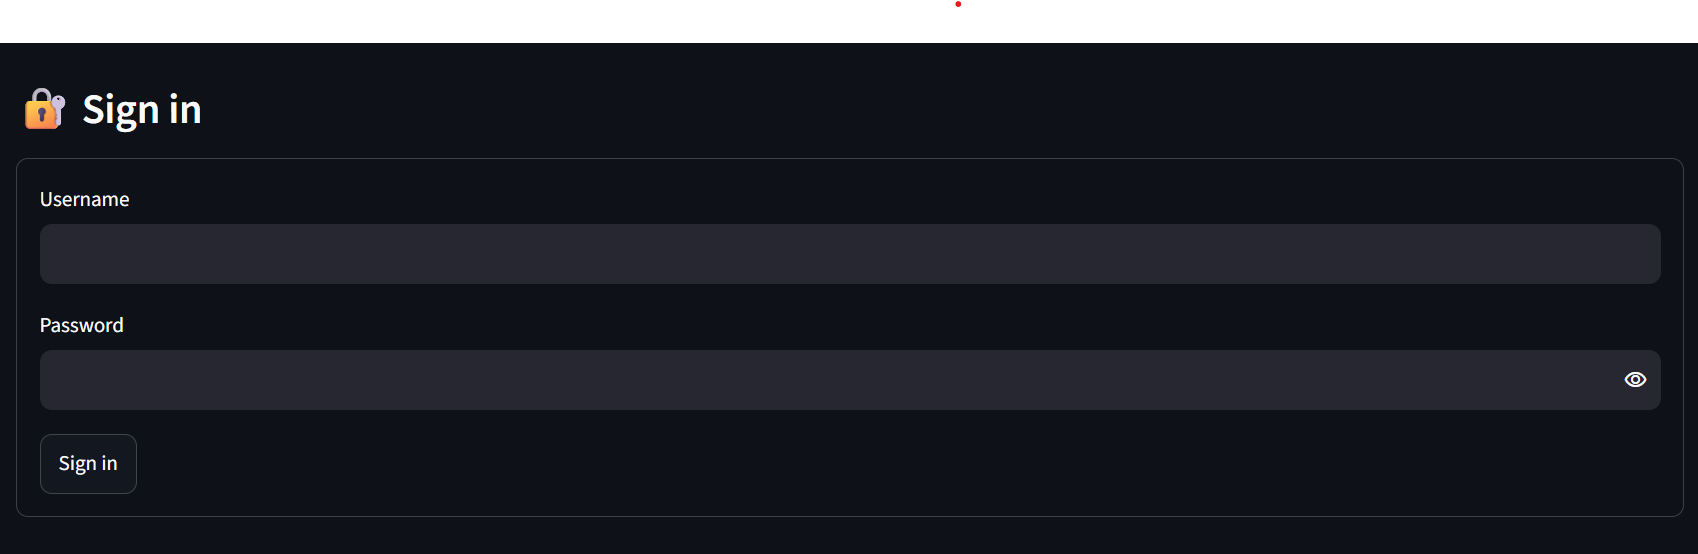
\includegraphics[
        width=0.95\linewidth,
        height=0.80\textheight,
        keepaspectratio
    ]{assets/frontend_login.png}
    \caption{Pantalla de inicio de sesión de la aplicación.}
    \label{fig:manual-login}
\end{figure}
\end{landscape}

\TFMAnnexSection{Inicio de una nueva propuesta}

Tras iniciar sesión, el usuario accede a la pantalla de conversación. Esta vista contiene
un campo de texto desde el que puede describir el viaje que desea preparar. El menú
lateral permite navegar entre la conversación con el orquestador y el histórico de
propuestas.

\begin{landscape}
\begin{figure}[H]
    \centering
    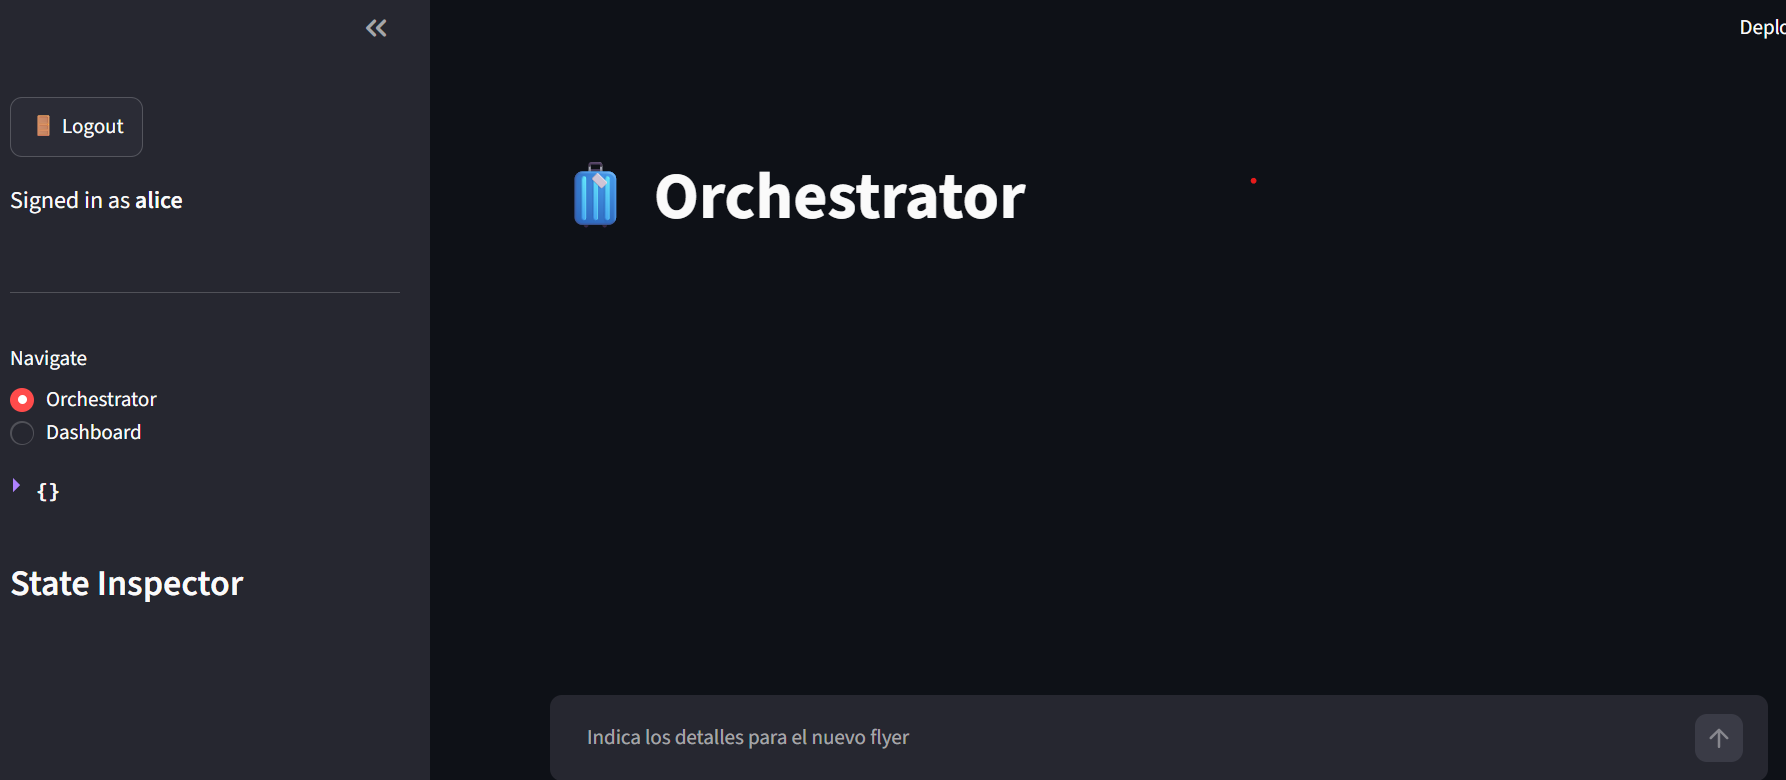
\includegraphics[
        width=0.95\linewidth,
        height=0.80\textheight,
        keepaspectratio
    ]{assets/image.PNG}
    \caption{Pantalla de conversación al iniciar una nueva sesión.}
    \label{fig:manual-orchestrator-vacio}
\end{figure}
\end{landscape}

El profesional introduce la petición en lenguaje natural, indicando datos como el
cliente, el origen, el destino, las fechas y los intereses del viaje. El agente
orquestador analiza el mensaje y solicita información adicional cuando alguno de los
parámetros necesarios no se encuentra disponible.

\begin{landscape}
\begin{figure}[H]
    \centering
    
\includegraphics[
        width=0.95\linewidth,
        height=0.80\textheight,
        keepaspectratio
    ]{assets/frontend_orchestrator_prompt.png}
    \caption{Ejemplo de petición de un viaje introducida en lenguaje natural.}
    \label{fig:manual-orchestrator-prompt}
\end{figure}
\end{landscape}

\TFMAnnexSection{Selección de vuelos y alojamiento}

Una vez recopilados los requisitos y consultadas las fuentes de información, el sistema
presenta distintas opciones de vuelos y alojamiento. Esta pantalla constituye el primer
punto de intervención humana del flujo.

El profesional debe seleccionar las alternativas que desea incorporar a la propuesta.
Las opciones pueden proceder de fuentes externas o de la documentación interna
indexada. La interfaz muestra la información disponible sobre horarios, escalas,
precios, valoraciones y características del alojamiento.

También se incluye una opción para indicar que el cliente se desplazará por sus propios
medios, evitando que sea necesario seleccionar un vuelo.

\begin{landscape}
\begin{figure}[H]
    \centering
    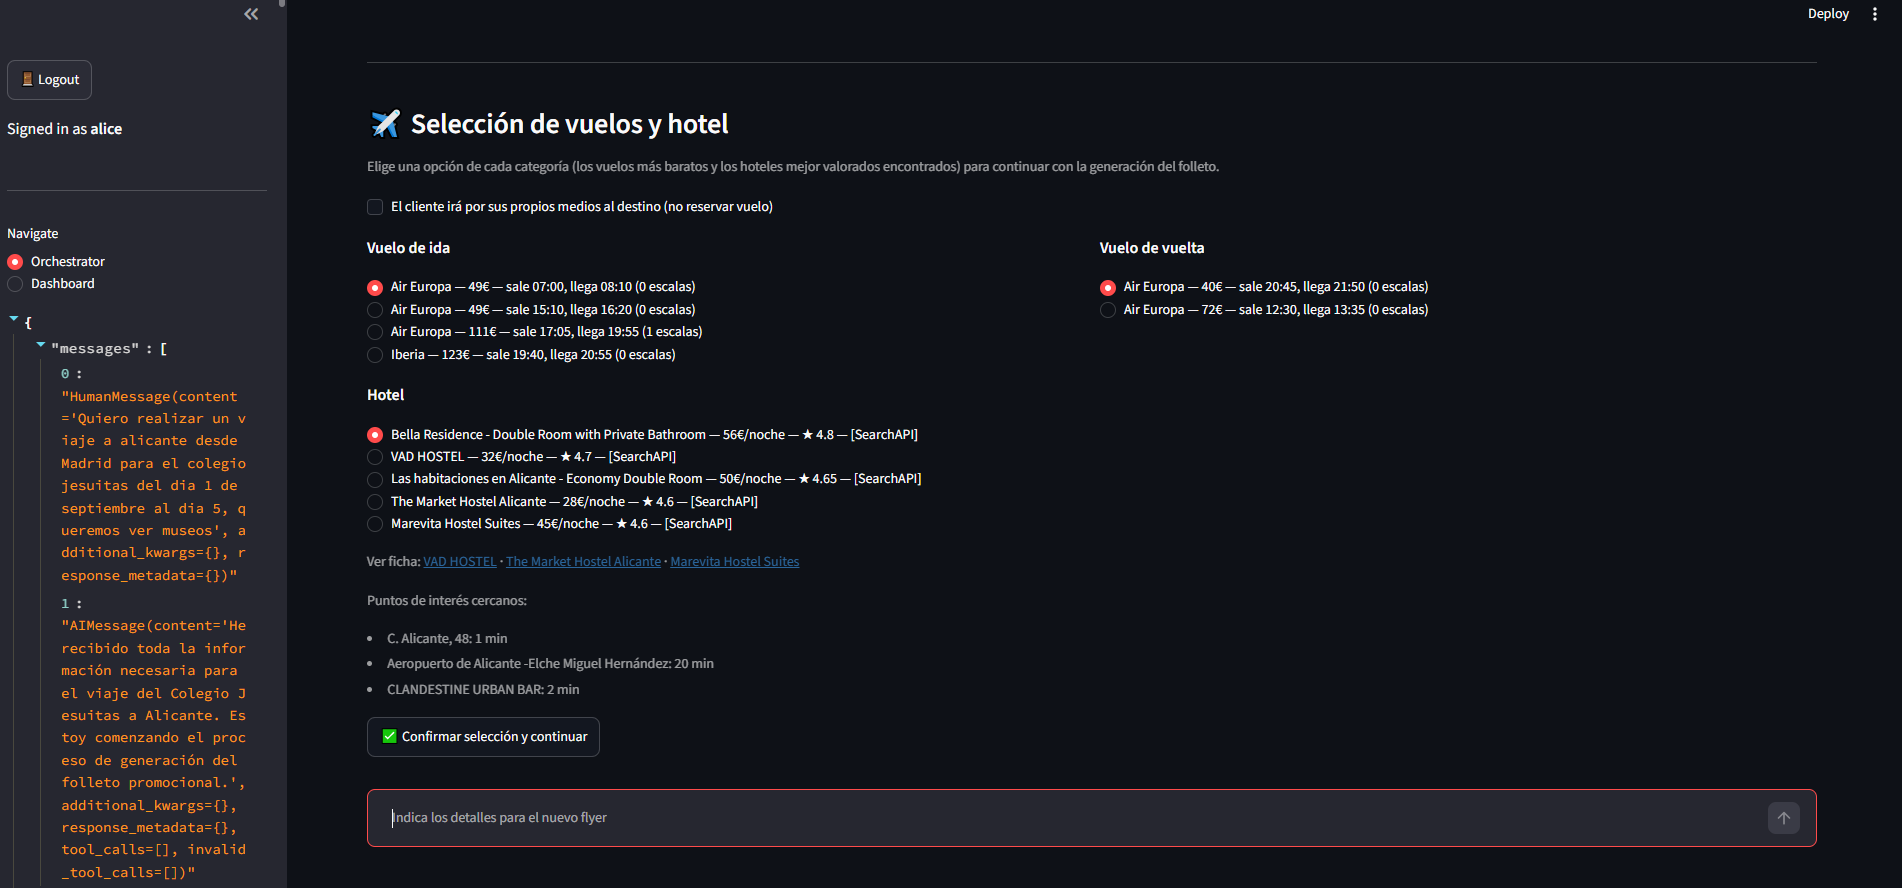
\includegraphics[
        width=0.95\linewidth,
        height=0.80\textheight,
        keepaspectratio
    ]{assets/frontend_seleccion_precios.png}
    \caption{Selección manual de vuelos y alojamiento.}
    \label{fig:manual-seleccion-precios}
\end{figure}
\end{landscape}

\TFMAnnexSection{Revisión de la propuesta comercial}

Después de seleccionar los precios, el sistema genera el itinerario, la imagen de portada
y la propuesta comercial en formato editable. Antes de finalizar el proceso, la
aplicación presenta un segundo punto obligatorio de revisión humana.

En esta pantalla, el profesional puede realizar las siguientes acciones:

\begin{tfmbullets}
    \item \textbf{Aprobar y publicar:} confirma que la propuesta puede considerarse
    finalizada.

    \item \textbf{Solicitar modificaciones:} permite introducir comentarios para
    corregir o regenerar el contenido.

    \item \textbf{Guardar como borrador:} conserva el estado actual para continuar
    posteriormente.

    \item \textbf{Descartar:} finaliza el proceso sin publicar la propuesta.
\end{tfmbullets}

\begin{landscape}
\begin{figure}[H]
    \centering
    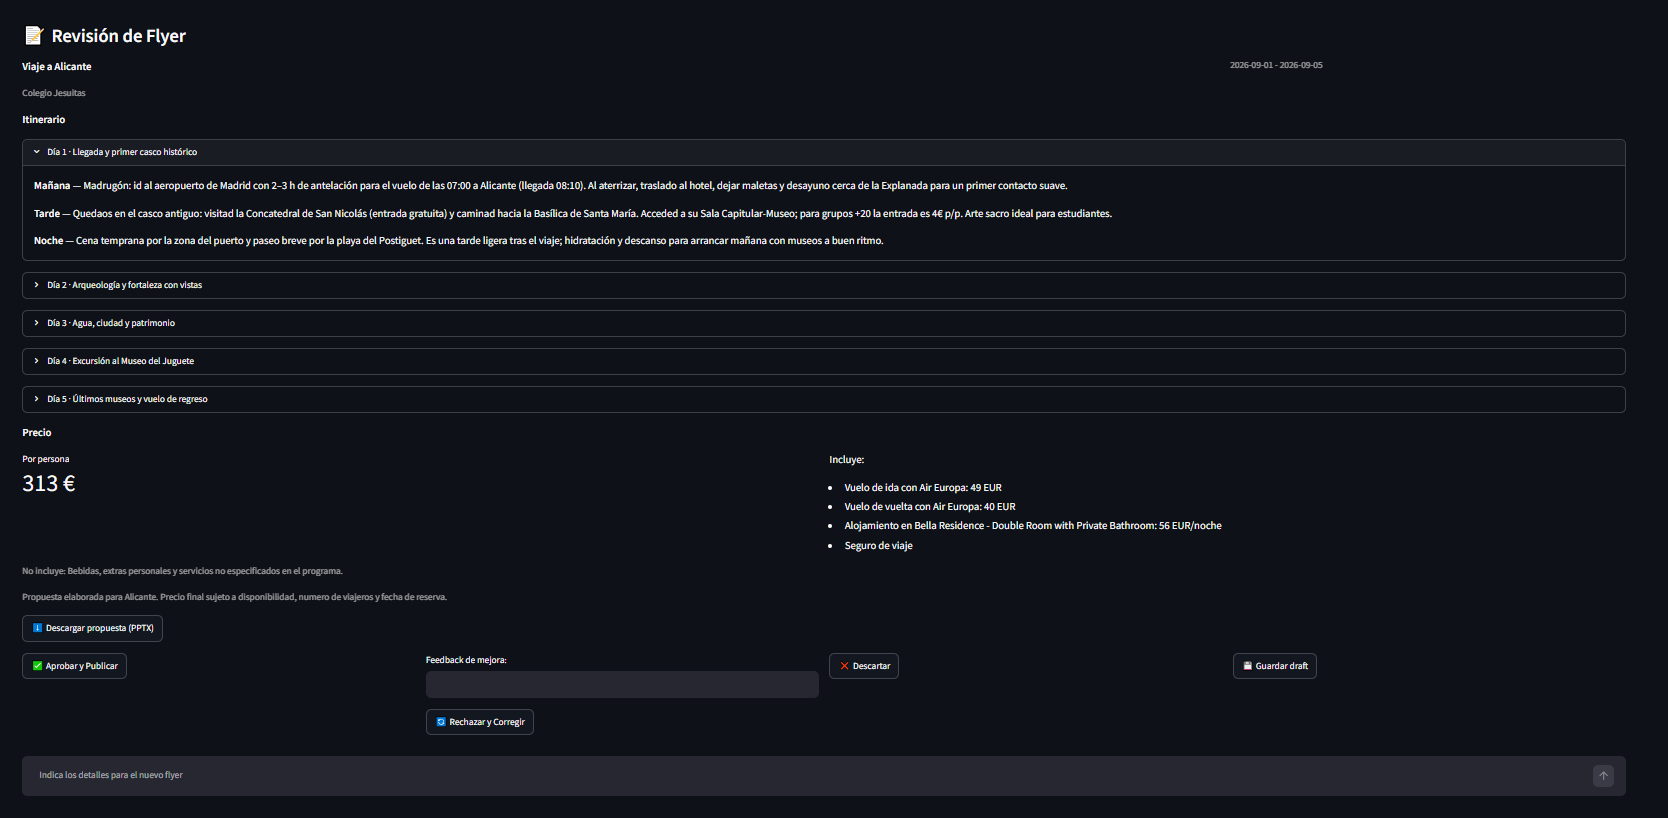
\includegraphics[
        width=0.95\linewidth,
        height=0.80\textheight,
        keepaspectratio
    ]{assets/frontend_revision_flyer.png}
    \caption{Pantalla de revisión final de la propuesta comercial.}
    \label{fig:manual-revision-flyer}
\end{figure}
\end{landscape}

\TFMAnnexSection{Histórico de propuestas}

La pantalla de histórico permite consultar las propuestas generadas por los distintos
miembros del equipo. La tabla muestra los principales datos de cada propuesta, como
el cliente, el origen, el destino, las fechas, los intereses, el estado y el usuario
responsable de su creación.

Esta vista facilita la recuperación de propuestas anteriores y permite conocer
rápidamente cuáles se encuentran en borrador, finalizadas, descartadas o pendientes
de revisión.

\begin{landscape}
\begin{figure}[H]
    \centering
    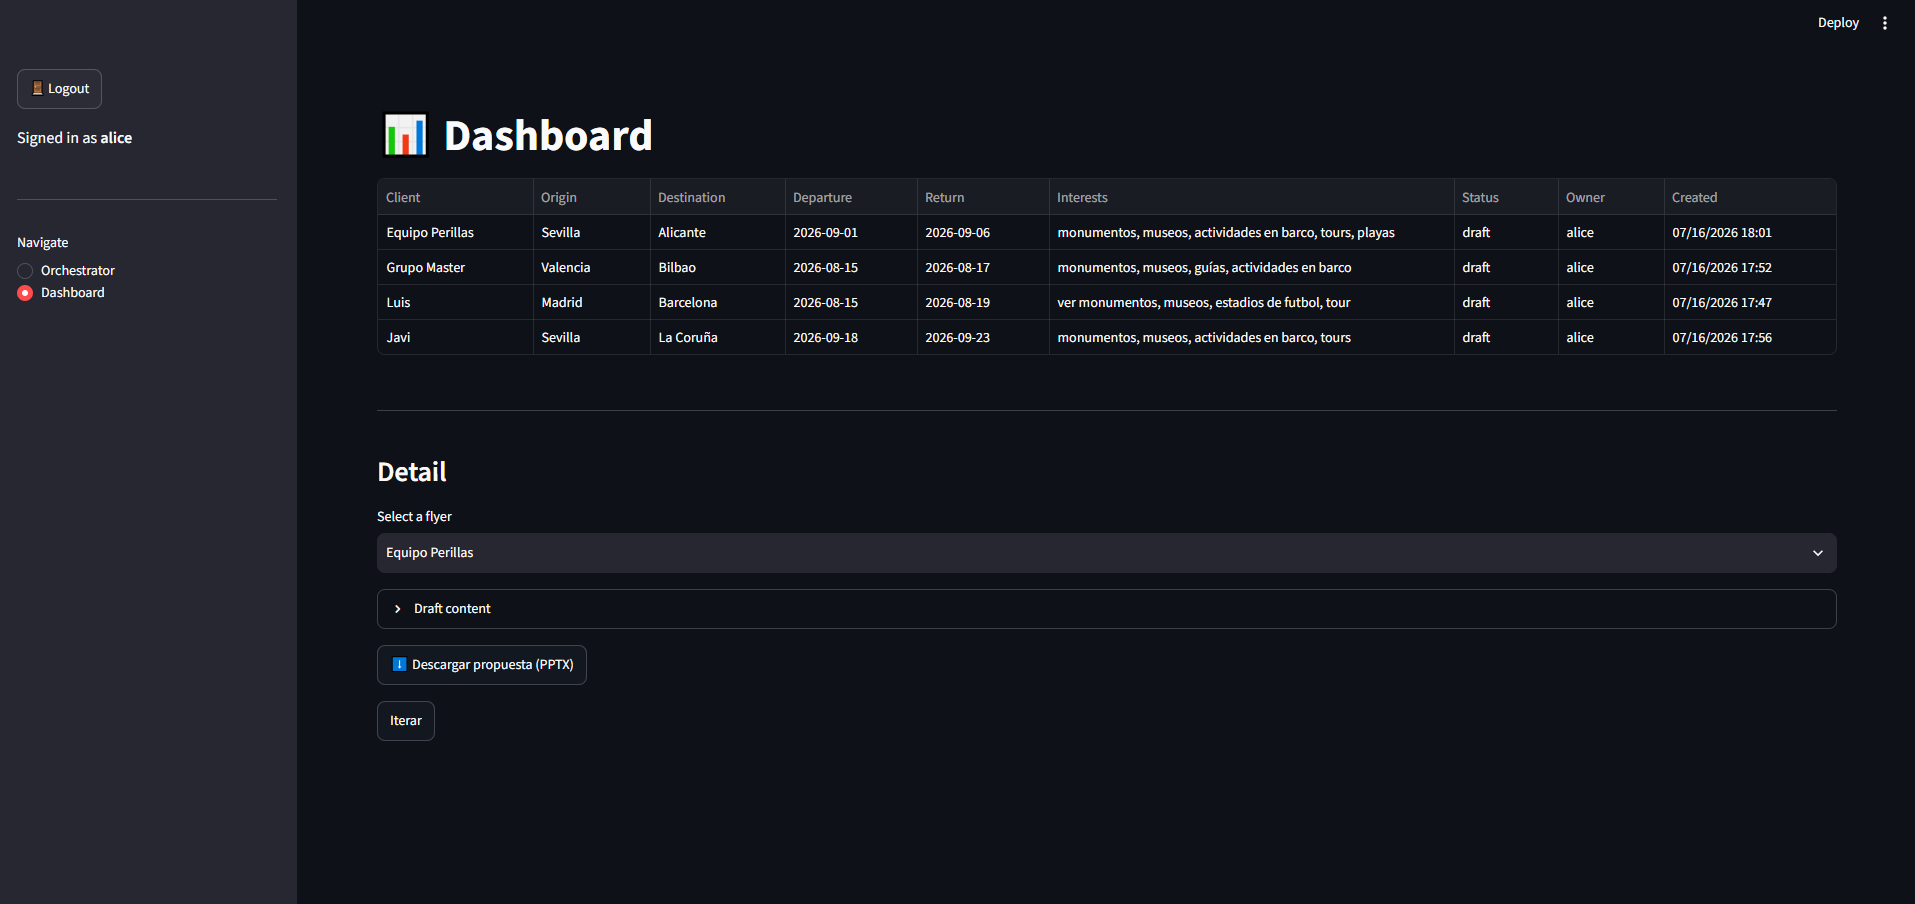
\includegraphics[
        width=0.95\linewidth,
        height=0.80\textheight,
        keepaspectratio
    ]{assets/frontend_dashboard.PNG}
    \caption{Pantalla de histórico con las propuestas generadas por el equipo.}
    \label{fig:manual-dashboard}
\end{figure}
\end{landscape}

\TFMAnnexSection{Consulta y descarga de una propuesta}

Al seleccionar una propuesta del histórico, la interfaz muestra su contenido disponible,
incluyendo los datos del viaje, el itinerario y el desglose del precio. Desde esta vista,
el profesional puede consultar el borrador, retomar su edición o descargar la propuesta
generada en formato PPTX.

El formato PowerPoint permite realizar modificaciones adicionales antes de entregar el
documento al cliente, manteniendo la propuesta generada como un contenido editable y
sujeto a revisión profesional.

\begin{landscape}
\begin{figure}[H]
    \centering
    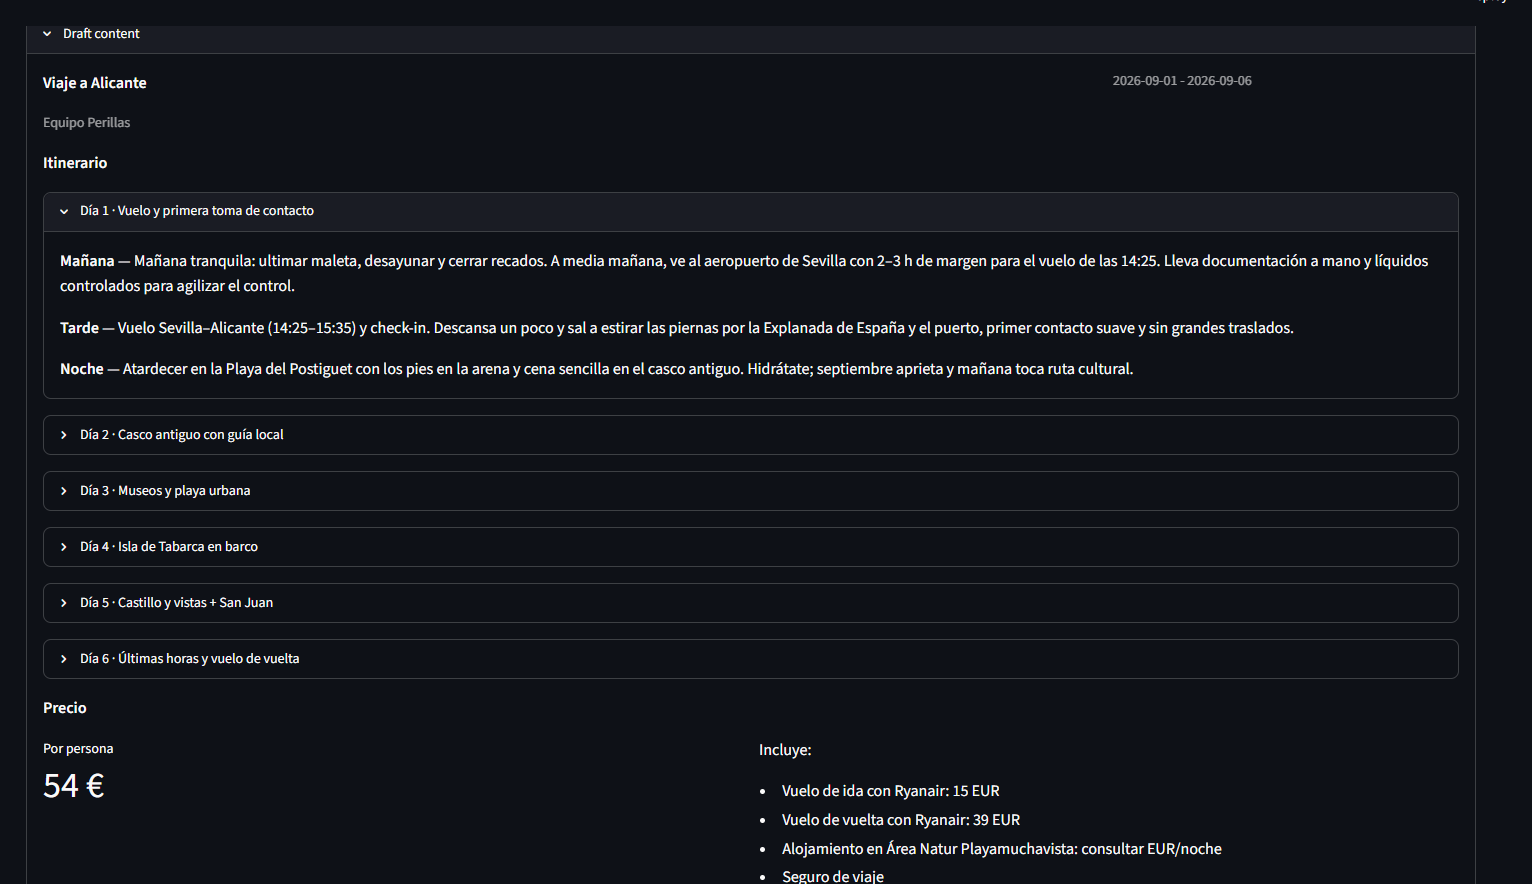
\includegraphics[
        width=0.95\linewidth,
        height=0.80\textheight,
        keepaspectratio
    ]{assets/frontend_dashboard_detalle.png}
    \caption{Detalle de una propuesta y opciones disponibles para el profesional.}
    \label{fig:manual-dashboard-detalle}
\end{figure}
\end{landscape}

\TFMAnnexSection{Flujo resumido de utilización}

El uso general de la aplicación puede resumirse en los siguientes pasos:

\begin{enumerate}
    \item El profesional inicia sesión en la aplicación.
    \item Introduce en lenguaje natural los requisitos del viaje.
    \item El sistema solicita los datos adicionales que resulten necesarios.
    \item Los agentes recuperan información turística y consultan vuelos y alojamientos.
    \item El profesional selecciona las opciones de precio que desea utilizar.
    \item El sistema genera el itinerario, la portada y la propuesta comercial.
    \item El profesional revisa el resultado y decide si aprobarlo, modificarlo,
    guardarlo como borrador o descartarlo.
    \item La propuesta queda disponible en el histórico y puede descargarse en formato
    PPTX.
\end{enumerate}

\TFMAnnexSection{Consideraciones de uso}

La aplicación desarrollada constituye una prueba de concepto y no realiza reservas,
pagos ni contrataciones de servicios turísticos. Los precios y la disponibilidad
consultados pueden variar, por lo que deben verificarse antes de presentar una oferta
definitiva al cliente.

Del mismo modo, el contenido generado por los modelos de inteligencia artificial debe
ser revisado por un profesional. La interfaz incorpora puntos de control humano
precisamente para evitar que una propuesta se publique o utilice sin una validación
previa.